\documentclass[UTF8,11pt]{ctexart}
\usepackage[a4paper,margin=2.3cm]{geometry}
\usepackage{amsmath,amssymb,amsthm}
\usepackage{booktabs}
\usepackage{graphicx}
\usepackage{float}
\usepackage[numbers]{natbib}
\usepackage{hyperref}
\usepackage{xcolor}
\usepackage{enumitem}
\usepackage{array}
\usepackage{longtable}
\usepackage{caption}
\graphicspath{{figures/}{figures/peak_shaving_diagnostics/}{figures/peak_shaving_submission/}{./}}
\hypersetup{colorlinks=true,linkcolor=blue,citecolor=blue,urlcolor=blue}
\captionsetup{font=small}
\setlength{\emergencystretch}{3em}

\newtheorem{proposition}{命题}
\newtheorem{remark}{评注}
\newtheorem{assumption}{假设}
\newtheorem{definition}{定义}
\newcommand{\qos}{q}
\newcommand{\T}{\mathcal{T}}
\newcommand{\M}{\mathcal{M}}
\newcommand{\D}{D}
\newcommand{\w}{\boldsymbol{w}}
\newcommand{\p}{\boldsymbol{p}}
\newcommand{\g}{\boldsymbol{g}}

\title{\textbf{固定算力约束下推理服务的分时动态定价：\\
异质厂家竞争、QoS保护与利润边界}}
\author{匿名作者}
\date{\today}

\begin{document}
\maketitle

\begin{abstract}
大模型推理服务在短期内受到固定GPU算力约束，而请求负载具有明显的日内峰谷差。高峰期过载会引起拥塞和服务质量（QoS）退化，低谷期则会造成算力闲置。本文研究固定算力约束下，分时动态定价是否能够通过高峰提价和低谷降价，引导时间弹性负载迁移，从而缓解拥塞并改善QoS。为此，本文构建了一个异质双厂家市场模型：两家厂家部署同款开源模型（如GLM），服务近似同质，算力规模不同；一个中间商在两家厂家之间路由流量；用户分为时间刚性和时间弹性两类，并可选择直连厂家API或退出市场。厂家的分时定价被低维形状参数化，厂家竞争通过虚拟博弈（fictitious play）求解。朴素最优响应在拥塞区间出现极限环振荡，虚拟博弈则给出可复现的时间平均策略；非拥塞区间跨随机种子的系统利润相对标准差为$4.31\times10^{-4}$。

结果表明，分时动态定价的QoS保护证据在多组诊断中保持一致。统一定价将最低QoS降至$0.756$，并将峰值利用率推至$0.782$；动态粗网格和细网格快照分别将峰值利用率降至$0.706$和$0.666$，并将最低QoS提高到$0.968$和$0.990$。为避免高regret细网格单快照导致误读，本文进一步在225点细网格上开展双重oracle混合策略诊断，得到$5\times5$支持的经验混合剖面；其完整细网格最大regret为$0.203$，期望峰值利用率为$0.703$，最低QoS为$0.970$。在容量、价格敏感度、迁移成本和QoS阈值的9个局部扰动场景中，最低QoS增益均为正，峰值利用率均下降。利润结果则不稳健：粗网格快照为$+9.3\%$，细网格快照为$-1.9\%$，低regret混合剖面约为$-2.8\%$。因此，本文将分时动态定价定位为固定算力约束下的QoS保护机制，而不是稳健的利润提升机制。所有经济参数均为合成标定；公开API价格和受控vLLM单卡测量分别只作为价格尺度和QoS退化形态锚点，不用于生产预测。
\end{abstract}

\noindent\textbf{关键词：}推理服务；动态定价；削峰填谷；异质厂家竞争；负载迁移；QoS保护；虚拟博弈；剩余重分配

% ============================================================
\section{引言}

\subsection{研究问题与动机}

大模型推理服务已经从离线批处理转向持续在线运行。交互式聊天、代码生成、自动代理、批量评测和定时工作流在日内呈现不同到达模式，GPU推理集群因此面临明显的峰谷差\cite{crankshaw2017clipper,gujarati2020clockwork,yu2022orca,kwon2023pagedattention,agrawal2024sarathiserve}。当利用率逼近容量上限时，首token延迟、排队时间和完成率都会迅速恶化。QoS退化进一步减少可结算服务量，并降低用户满意度。

与可快速调度供给或长期扩容的系统不同，GPU算力在短期内近似固定。采购和部署存在前置周期与沉没成本，低谷期闲置算力也仍产生持有成本。因此，推理服务商同时面临高峰拥塞和低谷闲置两个运营问题。一个可行的运营手段是在不扩容的前提下，通过价格信号重新分配可迁移负载的服务时段。

本文研究这一思路的一个具体版本：在固定算力约束下，厂家能否通过分时动态定价（高峰提价、低谷降价）将时间弹性负载从高峰转移到低谷，从而改善高峰期QoS。这一问题与电力市场实时定价和需求响应具有相似动机\cite{schweppe1988spot,borenstein2005long,albadi2008summary,faruqui2010household,siano2014demand}，但推理服务的关键约束不同。其服务质量取决于GPU局部利用率、延迟和完成率，而不是发电约束和网络潮流。

\subsection{竞争结构与异质算力}

现实中的推理服务市场通常并非单平台垄断。同一款开源模型（如GLM系列）可以由多家厂家部署，外部可感知的模型能力近似同质。竞争因此更多体现为价格、可用容量和QoS差异，而不是模型能力差异。这一设定为本文的厂家竞争提供了微观基础，也区别于单平台垄断定价模型。

厂家之间的算力规模也存在异质性。算力储备较小的厂家在承接路由流量时更容易进入拥塞区间，因此异质算力会改变动态定价和路由策略的可行空间。基于此，本文设定两家算力不同但服务同质的厂家，引入一个能够在两家之间路由流量的中间商（类似OpenRouter这类API聚合商），并允许用户绕开中间商直连厂家API，或者直接退出市场。

\subsection{相关文献与研究定位}

本文处在三条文献的交叉处。第一条是在线推理服务系统，已有工作主要解决低延迟、批处理、内存管理、模型并行和prefill/decode拆分等资源调度问题\cite{crankshaw2017clipper,gujarati2020clockwork,romero2021infaas,yu2022orca,li2023alpaserve,sheng2023flexgen,kwon2023pagedattention,agrawal2024sarathiserve,patel2024splitwise,zhong2024distserve,agrawal2024vidur}。这些工作刻画了QoS随利用率恶化的系统机制，但通常不把价格、退出和跨厂家竞争放进同一个市场模型。

第二条是动态定价、拥塞收费和收入管理。交通拥塞经济学和库存/容量受限收入管理已经长期研究价格如何在高需求时段分配稀缺容量\cite{vickrey1969congestion,arnott1990bottleneck,gallego1994dynamic,elmaghraby2003dynamic,bitran2003overview,talluri2004revenue,phillips2005pricing}；电力实时定价和需求响应则提供了削峰填谷的经典类比\cite{schweppe1988spot,borenstein2005long,allcott2011rethinking,siano2014demand}。本文借用了这类思想，但不把推理服务直接等同于电力或交通：GPU推理的QoS反馈、API退出选项和中间商路由会改变价格作用路径。

第三条是AI服务定价和平台经济学。近年的LLM价格研究开始讨论智能市场、菜单定价、token流清算和GPU云平台的Stackelberg定价\cite{demirer2025emerging,erdil2025inference,bergemann2025menu,guo2026prillm,yan2026stackelberg,cunningham2026token,liu2026locational}。本文的范围更窄，只研究固定算力、同质模型、双厂家和单中间商下的分时形状族。因此，本文的贡献不在于提出一般价格理论，而在于将QoS拥塞、退出选项和异质厂家竞争纳入同一个可复现实验框架。用户选择部分使用离散选择和平台市场的基本工具\cite{mcfadden1974conditional,anderson1992discrete,train2009discrete,rochet2003platform}。

\subsection{贡献}

\begin{enumerate}[leftmargin=2em]
  \item \textbf{固定算力约束下的削峰填谷动态定价模型。} 模型包含竞争的异质双厂家、可路由流量的中间商、时间刚性和时间弹性用户，以及一个外部退出选项。该框架同时刻画固定算力闲置成本、QoS拥塞退化和用户负载迁移。
  \item \textbf{可复现的形状族求解。} 厂家间竞争使用低维形状参数化和虚拟博弈（fictitious play）求解。朴素最优响应在拥塞区间会陷入极限环振荡；改用虚拟博弈后，非拥塞区间的跨种子系统利润相对标准差为$4.31\times10^{-4}$，拥塞区间则以regret作为可盈利偏离的诊断量。
  \item \textbf{带边界的QoS保护证据。} 粗、细两套网格和细网格混合策略诊断给出一个有边界的结论：拥塞时分时动态定价的削峰和QoS改善方向一致，但利润结果不稳健。本文据此将分时定价定位为可能的QoS保护工具，而不是利润提升机制，并明确给出求解、参数扫描和合成标定边界。
\end{enumerate}

% ============================================================
\section{模型}
\label{sec:model}

\subsection{市场结构与时序}

一天划分为$T$个时段$\T=\{1,\ldots,T\}$，每时段时长$h$。市场含：
\begin{itemize}[leftmargin=2em]
  \item \textbf{两个异质厂家} $\M=\{A,B\}$，固定算力$G_A>G_B$，部署同款开源模型（服务同质）。厂家$m$选择分时批发价$w_{m,t}$（卖给中间商）和分时直连零售价$p^D_{m,t}$（卖给用户）。
  \item \textbf{一个中间商}，观察批发价后选择对用户的分时零售价$p_t$和把每时段流量分配给两厂家的路由权重$r_{m,t}$（$\sum_m r_{m,t}=1$）。
  \item \textbf{两类用户}，按logit随机效用在"中间商通道、厂家A直连、厂家B直连、退出"之间选择。
\end{itemize}
时序为：厂家同时出价（Nash竞争）$\to$ 中间商最优响应 $\to$ 用户选择与QoS拥塞固定点。

\begin{figure}[H]
\centering
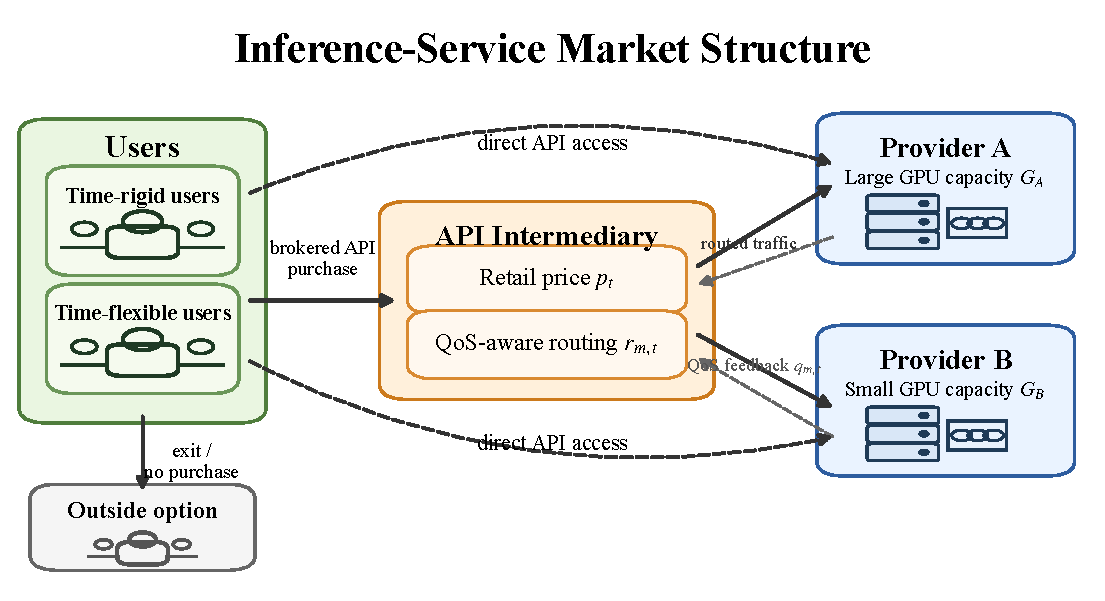
\includegraphics[width=0.82\textwidth]{market_schematic.pdf}
\caption{市场结构：用户可经中间商、厂家直连或退出；中间商根据批发价和QoS在两家厂家之间路由。}
\label{fig:market_schematic}
\end{figure}

\subsection{两类用户与外部退出选项}

设用户类型$\theta\in\{R,E\}$，$R$为时间刚性、$E$为时间弹性。类型$\theta$对通道$k$（中间商/厂家A/厂家B）在时段$t$的确定性效用为
\begin{equation}
  z^\theta_{k,t}=\log b_k+\log a_t
  -\alpha_\theta\!\left[\text{price}_{k,t}+c_s^\theta(1-\pi^\theta_t)-p_0\right]
  -\gamma(1-q_{k,t}),
  \label{eq:utility}
\end{equation}
其中$b_k$为通道品牌或便利性，$a_t$为时段偏好，$\pi^\theta_t$为类型$\theta$的原生时段分布，$q_{k,t}$为通道QoS。迁移成本被写入价格化的广义成本，因此会和价格一起受到$\alpha_\theta$缩放；这与仿真实现中的效用口径一致。两类用户的差别全部落在参数上：刚性用户价格敏感度$\alpha_R$低、迁移成本$c_s^R$高、原生时段挤在高峰；弹性用户则$\alpha_E$高、$c_s^E$低、原生时段比较分散。

logit归一化中加入一个确定效用为$u_0$的no-purchase外部退出选项。类型$\theta$选通道$k$时段$t$的份额，以及退出概率，分别为
\begin{equation}
  s^\theta_{k,t}=\frac{\exp(z^\theta_{k,t})}{\exp(u_0)+\sum_{k',t'}\exp(z^\theta_{k',t'})},
  \qquad
  s^\theta_0=\frac{\exp(u_0)}{\exp(u_0)+\sum_{k',t'}\exp(z^\theta_{k',t'})}.
  \label{eq:share}
\end{equation}
内部份额之和小于1，剩余质量$s^\theta_0$表示真实退出概率，不会被重新分配给内部选项。因此，当价格上升时，部分需求会离开市场，而不是在归一化过程中被重新摊回可购买选项。

\subsection{需求、负载与QoS}

类型$\theta$对通道$k$的需求由弹性项和刚性/重放项构成，二者均\textbf{按渠道自身份额}分配（使每时段刚性总量与渠道数无关）：
\begin{equation}
  \D^\theta_{k,t}=\bar F_\theta\,m(\p)\,s^\theta_{k,t}
  +\bar R^\theta_t\,\sigma[\beta(v_r-\text{price}_{k,t})]\,s^\theta_{k,t}.
  \label{eq:demand}
\end{equation}
总需求为两类人口加权之和，权重$(\pi_R,\pi_E)$。需要注意，本文不是严格固定总需求模型：退出选项允许内部需求减少，弹性市场规模项$m(\p)$允许低价时需求扩张。因此，后文关于利润边界的解释是机制分解和数值诊断，而不是建立在固定总需求假设上的定理。厂家$m$在时段$t$的总负载为直连需求加中间商按路由分来的需求：
\begin{equation}
  L_{m,t}=\D^D_{m,t}+r_{m,t}\,\D^I_t,\qquad u_{m,t}=L_{m,t}/G_m,\qquad q_{m,t}=\qos(u_{m,t}).
  \label{eq:load}
\end{equation}
QoS退化函数$\qos(u)$在利用率越过阈值$\bar u$之后开始下降。由于$G_B<G_A$，同样的负载分配给厂家$B$时更容易越过阈值并进入拥塞区间。主实验使用平滑的sigmoid退化形态；阈值型、线性和根号型三种形态用于鲁棒性检验。

\subsection{利润：把固定算力的闲置成本算进去}

厂家$m$的利润等于批发收入加直连收入，再减去按固定算力计的闲置成本和QoS退化成本：
\begin{equation}
  \Pi_m=h\!\sum_t\! w_{m,t}r_{m,t}\D^I_t q_{m,t}
  +h\!\sum_t\! p^D_{m,t}\D^D_{m,t}q_{m,t}
  -h\!\sum_t\! c_g G_m
  -h\!\sum_t\! c_q(1-q_{m,t})L_{m,t}.
  \label{eq:firm_profit}
\end{equation}
闲置成本$c_g G_m$按固定算力计提，与短期利用率无关。该项成本为厂家降低低谷价格、提高低谷利用率提供了动机，也使本文区别于仅将容量设为常数且不计闲置成本的模型。中间商利润等于零售收入减批发成本再减QoS退化成本。系统利润定义为两家厂家利润与中间商利润之和。


% ============================================================
\section{均衡求解}
\label{sec:solver}

\subsection{低维定价形状族}

如果每个厂家直接在$2T$维（分时批发价加直连价）的连续空间中优化，Nash求解会同时面临高维、非凸和数值可复现性问题。本文因此将厂家的分时定价限制在低维形状族内：
\begin{equation}
  w_{m,t}=\bar w_m\big(1+\delta_m\,\widehat{\ell}_t\big),\qquad
  p^D_{m,t}=\bar p^D_m\big(1+\delta^D_m\,\widehat{\ell}_t\big),
  \label{eq:shape}
\end{equation}
其中$\widehat{\ell}_t$是零均值的标准化负载形状，由刚性需求基线归一化得到，并作为外生输入给定。每个厂家的策略由四个标量$(\bar w_m,\delta_m,\bar p^D_m,\delta^D_m)$表示。$\delta_m=0$对应统一定价，$\delta_m>0$对应高峰提价。该参数化牺牲了连续全空间最优性，但换取了可复现和可诊断的求解过程。因此，本文仅讨论形状族内的均衡近似，不声称求得$2T$维连续策略空间的全局最优。

\subsection{虚拟博弈与低exploitability诊断}

厂家的最优响应通过四标量空间上的网格搜索计算。网格搜索对非光滑QoS目标更稳健，计算成本可预测，也便于并行复核。中间商响应同样使用网格搜索；每次评估内嵌一个QoS和路由的联合固定点，并通过阻尼迭代求解。本文没有使用更深层的嵌套连续优化，因为该方案在拥塞区间会显著增加计算成本。

朴素最优响应迭代（厂家轮流对对手当前策略做最优响应）在拥塞区间会出现周期性振荡，策略在两组配置之间反复切换，形成极限环。这类现象在寡头定价博弈中并不少见。本文改用虚拟博弈：每个厂家对对手的运行平均策略而非当前策略做最优响应，并利用历史平均缓解振荡。输出对象因此不是未经限定的纯策略Nash均衡，而是形状族内的虚拟博弈时间平均策略。只有当最大单边偏离收益（regret）足够低时，本文才将其视为可接受的均衡近似。本文不以参数漂移作为主要收敛判据，因为该指标在粗网格下可能给出虚假的收敛信号。对细网格，本文进一步补充双重oracle诊断：从少量候选策略开始，在完整225点细网格中反复加入对当前混合剖面的最优偏离，并在受限支持上用经验虚拟博弈求混合剖面，最后用完整细网格扫描regret。

\begin{remark}[收敛性与诚实边界]
非拥塞区间中，QoS恒为1，固定点一步收敛，网格求解完全确定，跨随机种子的系统利润相对标准差为$4.31\times10^{-4}$。拥塞区间需要单独处理。粗网格下虚拟博弈的regret单调下降（$133.6\to63.7\to\cdots\to4.98$，22轮达到regret$<5$）；但在细网格单快照下，regret在第10轮左右触底于$\approx14$之后不降反升，40轮后漂移至$\approx22$。新增的双重oracle混合诊断在完整225点细网格上得到$5\times5$支持的混合剖面，最终最大regret为$0.203$。因此，本文可以把QoS改善作为有限细网格混合/平均策略意义下的低exploitability诊断结果；但这仍不是连续$2T$维策略空间的全局均衡定理。
\end{remark}

% ============================================================
\section{实验结果}
\label{sec:results}

\subsection{设置}

$T=8$时段、$h=3$小时。基准算力$G_A=1500,G_B=600$；拥塞情形将算力收紧至$G_A=300,G_B=120$以激活QoS退化。两类用户人口占比基准$(\pi_R,\pi_E)=(0.6,0.4)$；拥塞情形取$(0.4,0.6)$以加大高峰压力。所有经济参数为合成标定，具体数值仅支撑机制方向，不作生产预测。作为价格尺度参照，我们核验了公开API价格：Z.AI的GLM-4.7为每百万token输入\$0.6、输出\$2.2，DeepSeek-chat为cache-miss输入\$0.27、输出\$1.10，OpenAI GPT-4o为输入\$2.50、输出\$10.00\cite{zaiPricing2026,deepseekPricing2026,openaiGpt4oPricing2026}。这些公开价格只说明本文归一化价格落在真实API数量级附近，不用于估计需求弹性。完整参数见补充材料。

为给QoS退化函数提供测量锚点，我们还复用两组受控vLLM单GPU过载测量。后端为vLLM 0.22.0，硬件为NVIDIA GeForce RTX 4090，模型为Qwen2.5-0.5B-Instruct和Qwen2.5-3B-Instruct；每个并发水平重复5次，QoS观测量定义为首token延迟不超过0.5秒的SLA达标率。图~\ref{fig:vllm_qos_anchor} 显示，两组测量在归一化并发不超过1时SLA达标率保持为1；超过健康并发后开始下降。0.5B模型在归一化并发1.71和2.29处的SLA达标率分别为0.635和0.500；3B模型在1.71处为0.667。用阈值型函数$q(u)=\exp[-\kappa(u-\bar u)^2_+]$拟合后，0.5B剖面的$(\bar u,\kappa,\mathrm{RMSE})=(1.000,0.517,0.068)$，3B剖面为$(1.058,0.942,6.3\times10^{-10})$。这说明本文使用的QoS代理具有受控后端测量中的阈值退化形态锚点；它仍不替代真实请求轨迹、用户弹性或生产SLA校准。

\begin{figure}[H]
\centering
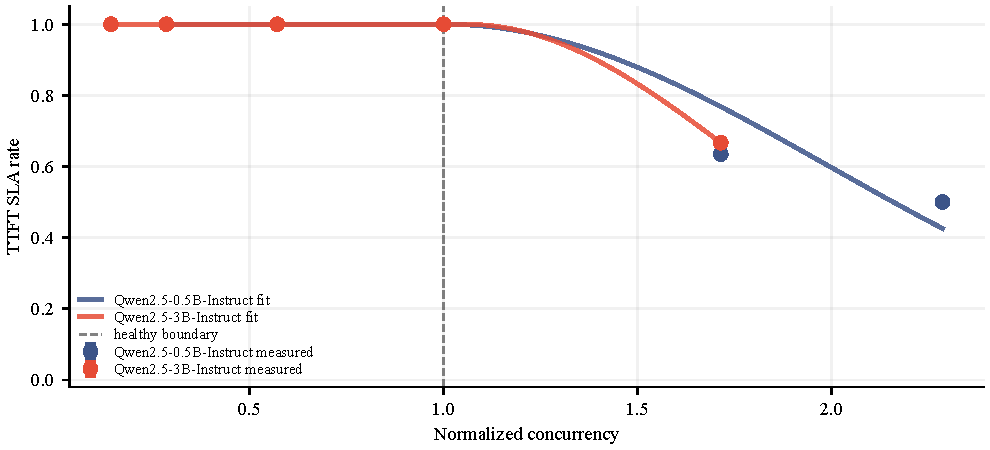
\includegraphics[width=0.88\textwidth]{vllm_qos_anchor.pdf}
\caption{受控vLLM单GPU过载测量给出的QoS退化锚点。横轴为相对最大健康并发归一化后的并发强度，纵轴为0.5秒首token延迟SLA达标率；点为5次重复测量均值，线为阈值型QoS函数拟合。}
\label{fig:vllm_qos_anchor}
\end{figure}

\subsection{非拥塞区间：负载迁移存在但利润效应有限}

基准算力下市场并不拥塞（统一定价的峰值利用率才$0.213$），QoS一直是1。表~\ref{tab:uncongested} 给出统一和动态定价的对比。

\begin{table}[H]
\centering
\caption{非拥塞区间：统一定价 vs 动态定价（确定性网格求解）}
\label{tab:uncongested}
\begin{tabular}{lccc}
\toprule
指标 & 统一定价 & 动态定价 \\
\midrule
系统利润 & 1193.3 & 1139.4 \\
峰值利用率 & 0.213 & 0.261 \\
弹性需求时段重心位移 & \multicolumn{2}{c}{$+0.177$} \\
刚性需求时段重心位移 & \multicolumn{2}{c}{$+0.077$} \\
\bottomrule
\end{tabular}
\end{table}

\textbf{负载迁移（P1）保持稳定。} 动态定价下弹性需求的时段重心后移$+0.177$，刚性需求后移$+0.077$。弹性需求的迁移强度约为刚性需求的$2.3$倍，与“动态定价主要驱动时间弹性负载”的机制判断一致。然而，非拥塞区间的QoS本来维持在1，QoS改善空间有限。动态定价的利润效应在中性到微负之间，弹性占比扫描下增益依次为$0\%,-0.32\%,-4.51\%,-3.76\%,-3.00\%$。这表明，分时动态定价发挥QoS保护作用的前提是市场进入拥塞区间。

\subsection{拥塞区间：QoS证据增强，利润仍不稳健}

把算力收紧之后，统一定价使市场进入拥塞区间。表~\ref{tab:congested} 并列报告统一定价基准、动态定价粗网格时间平均策略、动态定价细网格单快照和细网格混合策略诊断，用来区分哪些结论依赖求解分辨率，哪些结论在更低exploitability的有限细网格混合剖面下仍然成立。

\begin{table}[H]
\centering
\caption{拥塞区间：统一 vs 动态定价（虚拟博弈时间平均、快照与混合策略诊断）}
\label{tab:congested}
\small
\begin{tabular}{lcccc}
\toprule
指标 & 统一定价 & 动态粗网格 & 动态细网格快照 & 细网格混合诊断 \\
\midrule
峰值利用率 & 0.782 & 0.706 & 0.666 & 0.703 \\
最低QoS & 0.756 & 0.968 & 0.990 & 0.970 \\
系统利润 & 1783 & 1949 & 1749 & 1733 \\
利润变化 & --- & $+9.3\%$ & $-1.9\%$ & $-2.8\%$ \\
max regret & --- & 4.98 & 22.30 & 0.203 \\
\bottomrule
\end{tabular}
\end{table}

\begin{table}[H]
\centering
\caption{拥塞区间证据边界}
\label{tab:evidence_boundary}
\small
\begin{tabular}{p{0.25\textwidth}p{0.28\textwidth}p{0.36\textwidth}}
\toprule
对象 & 求解状态 & 本文允许使用的结论 \\
\midrule
统一定价基准 & 虚拟博弈收敛，10轮内达到判据 & 作为拥塞基准使用。 \\
动态定价粗网格 & 22轮后regret为$4.98$，但粗网格会掩盖更细偏离 & 可作为低分辨率诊断，不单独支撑定量利润结论。 \\
动态定价细网格快照 & 40轮后最大regret约$22.3$，未达到$<5$判据 & 只作为分辨率压力测试和方向对照，不作为均衡定量结论。 \\
细网格混合诊断 & 完整225点细网格扫描下最大regret为$0.203$ & 支撑有限细网格混合/平均策略意义下的QoS结论；不外推到连续策略空间。 \\
\bottomrule
\end{tabular}
\end{table}

\begin{figure}[H]
\centering
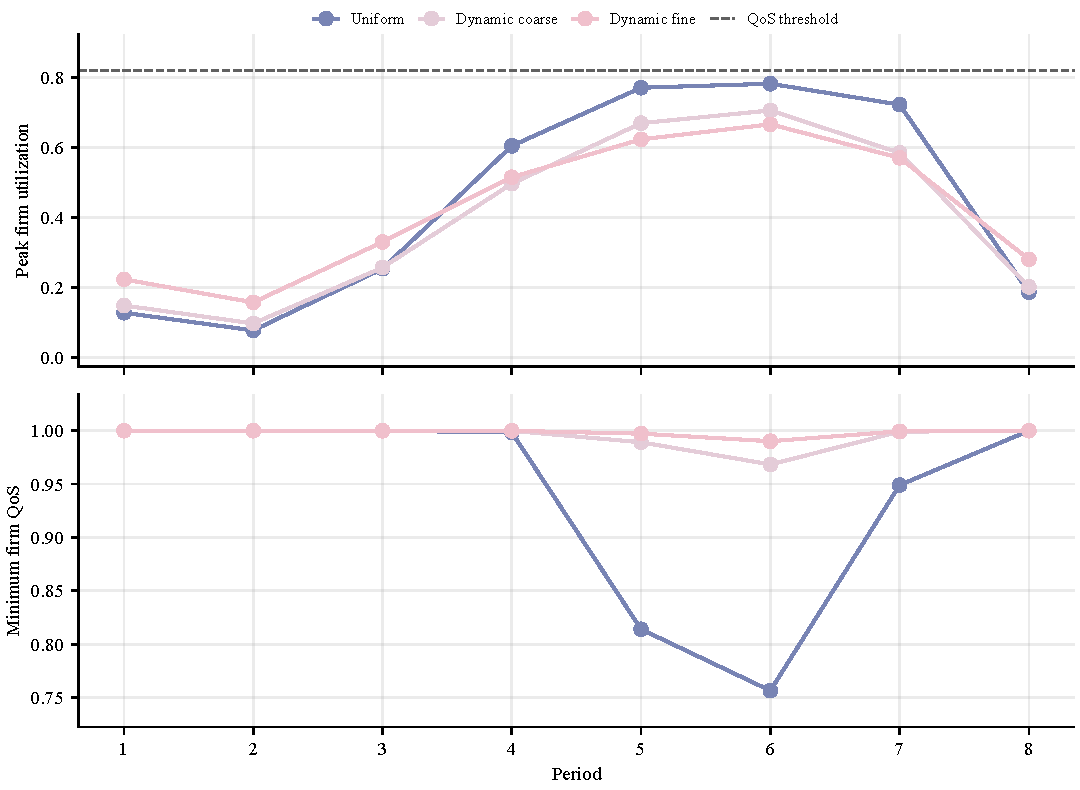
\includegraphics[width=0.86\textwidth]{qos_utilization_profiles.pdf}
\caption{拥塞区间的时段利用率与QoS剖面。动态策略在粗、细两套快照中都把峰值利用率压低，并把最低厂家QoS拉回阈值附近或以上。}
\label{fig:qos_profiles}
\end{figure}

\begin{figure}[H]
\centering
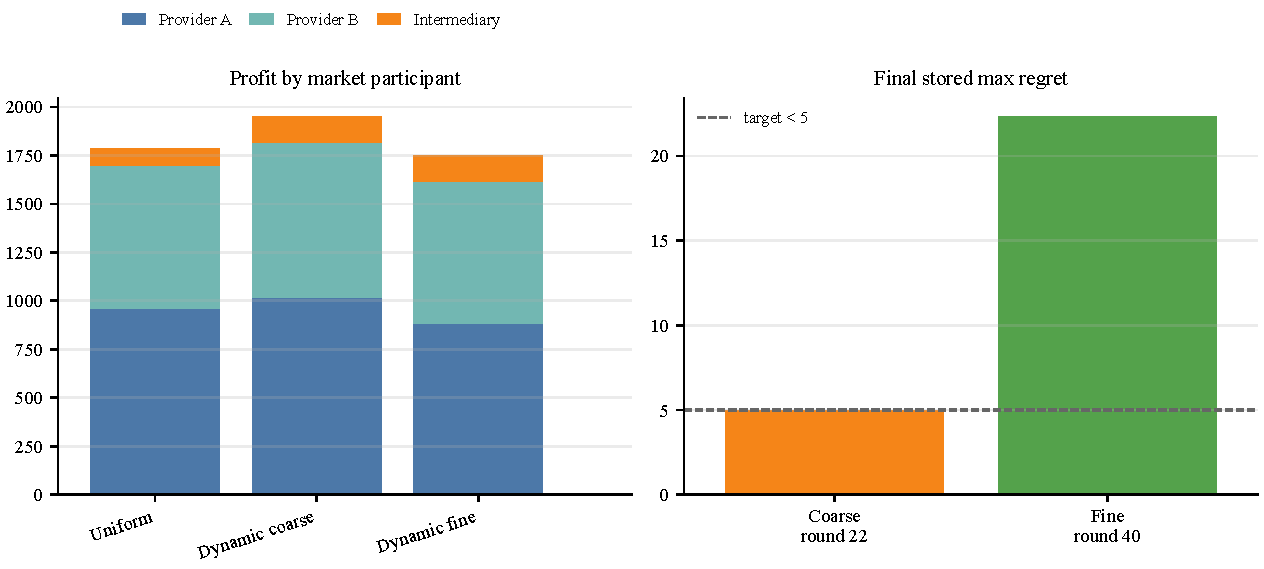
\includegraphics[width=0.88\textwidth]{profit_components_and_regret.pdf}
\caption{利润分布与单快照收敛边界。粗网格最终regret低于5，但细网格第40轮仍为$22.3$，因此细网格单快照的利润和策略强度不能作为稳健均衡结论。}
\label{fig:profit_regret}
\end{figure}

\begin{figure}[H]
\centering
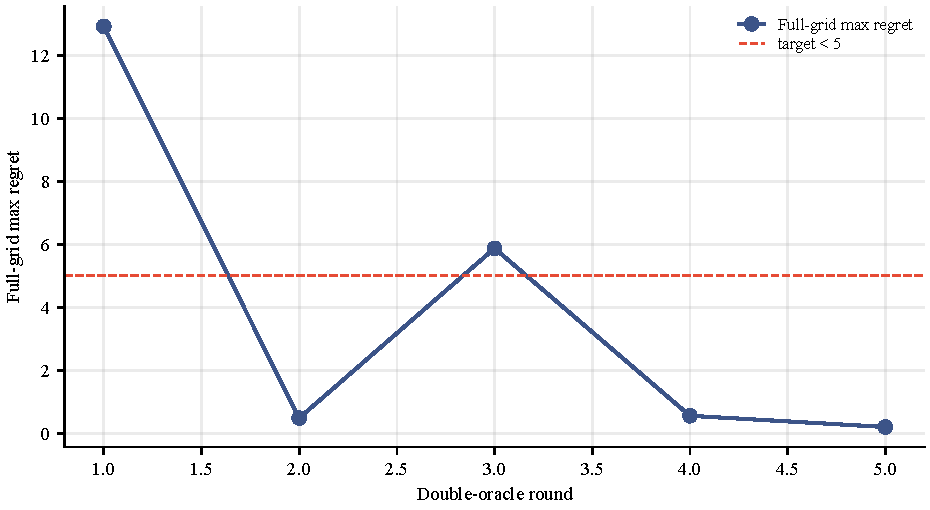
\includegraphics[width=0.76\textwidth]{mixed_oracle_regret.pdf}
\caption{细网格双重oracle混合策略诊断。每轮在完整225点细网格中加入当前混合剖面的最优偏离；第5轮得到$5\times5$支持，完整细网格最大regret降至$0.203$。}
\label{fig:mixed_oracle}
\end{figure}

\textbf{QoS改善方向在快照和混合剖面下都成立。} 统一定价把最低QoS压到$0.756$，峰值利用率推到$0.782$。动态定价快照把峰值利用率降到$0.66$--$0.71$，最低QoS拉回$0.97$--$0.99$；细网格混合策略诊断的期望峰值利用率为$0.703$，最低QoS为$0.970$。因此，QoS结果不再只依赖未收敛的细网格单快照，而是在有限细网格混合/平均策略意义下也得到低regret支持。

\textbf{没有观察到稳健的正利润效应。} 系统利润变化在粗网格下为$+9.3\%$，在细网格快照下变为$-1.9\%$，在低regret混合剖面下约为$-2.8\%$。因此，本文不将利润变化作为正向发现。更稳健的解释是：在当前求解预算和形状族内，分时动态定价显示出QoS保护价值，但没有显示出稳健的正利润增益。

\textbf{厂家差异假设没有得到稳定支持。} 一个自然假设是，算力较小的厂家可能更依赖动态定价，即$\delta_B>\delta_A$。但粗网格给出$\delta_A=0.383$、$\delta_B=0.023$，细网格给出$\delta_A=0.059$、$\delta_B=0.278$，方向随网格分辨率变化而翻转。因此，本文不保留关于哪类厂家更动态的结论。负载迁移的非对称性（P1）也类似：非拥塞区间较清楚，在拥塞求解对象下则明显削弱。细网格下弹性和刚性需求重心分别为$4.23$和$4.31$，差异很小。

\subsection{局部参数压力测试}

为检验QoS方向是否只来自单一合成标定，我们围绕拥塞基准做四组局部扰动：容量规模、价格敏感度、迁移成本和QoS阈值。每个扰动点不重新求解均衡，而是评估已报告的统一、动态粗网格和动态细网格策略快照。因此，它是固定策略的压力测试，不是跨参数均衡命题。

\begin{figure}[H]
\centering
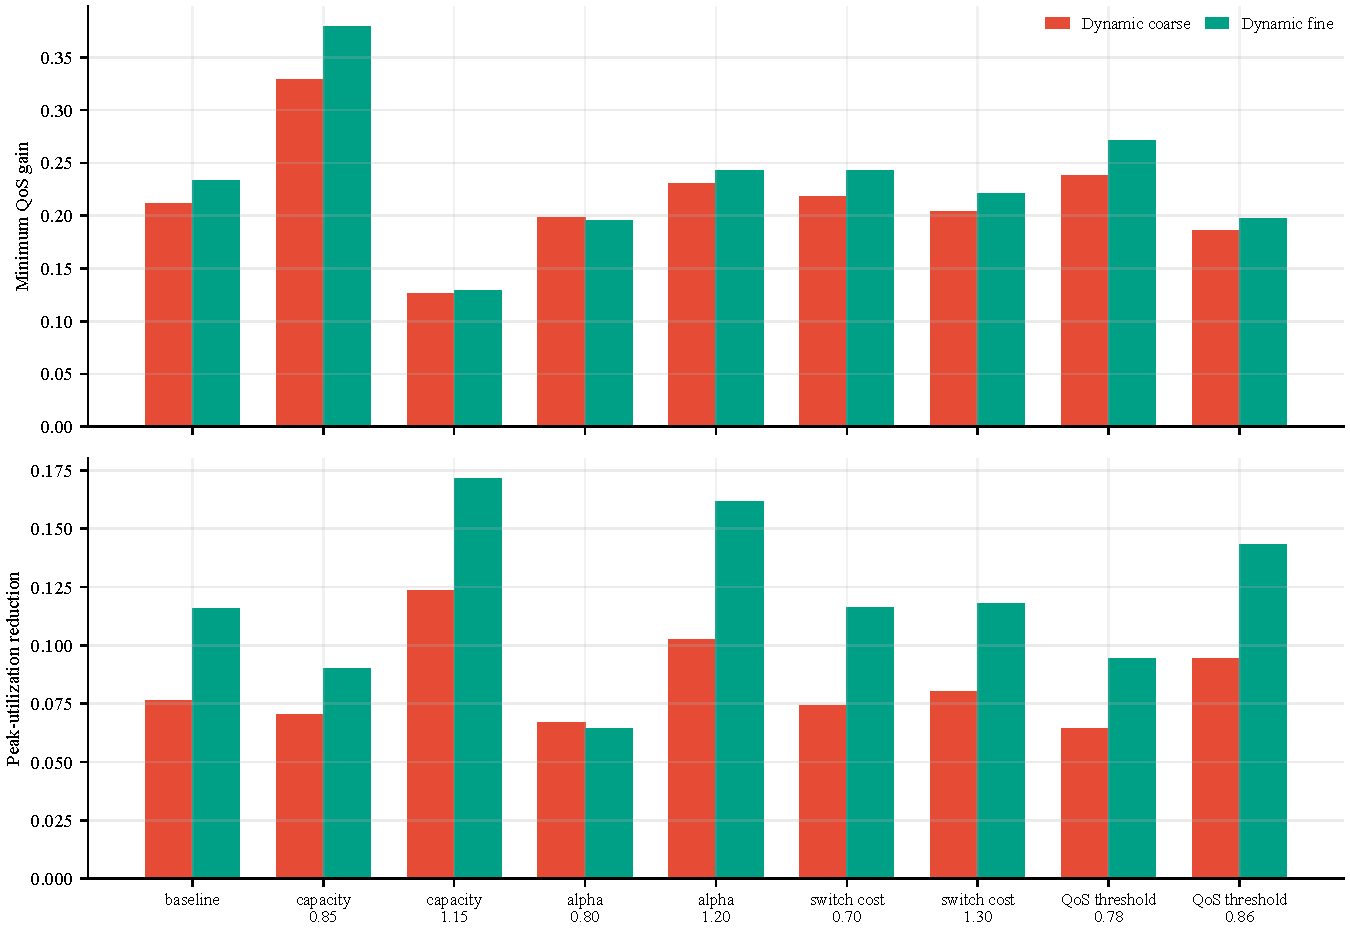
\includegraphics[width=0.92\textwidth]{parameter_sweep_qos.pdf}
\caption{参数压力测试。9个扰动场景下，动态粗网格和动态细网格快照相对统一定价均保持正的最低QoS增益和峰值利用率下降。}
\label{fig:parameter_sweep}
\end{figure}

图~\ref{fig:parameter_sweep} 显示，动态粗网格和动态细网格快照在9个扰动场景中均保持正的QoS增益和峰值利用率下降；最低QoS增益的最小值分别为$0.126$和$0.129$。利润结果仍然不应强化：粗网格在9个场景中利润增益为正，但细网格只有1个场景为正。这组扫描因此增强了“QoS方向”的泛化证据，同时再次说明“利润提升”不是稳健结论。

% ============================================================
\section{讨论：QoS改善与利润边界}
\label{sec:discussion}

拥塞区间的主要现象是，QoS显著改善（从$0.756$升至$0.97$左右或以上），但利润没有形成稳健的正向结果。由于利润符号在粗网格、细网格快照和低regret混合剖面之间不一致，本文不将利润数值作为正向结论，而将其作为机制诊断，用以解释QoS改善为何并不必然转化为厂家利润增长。

\begin{figure}[H]
\centering
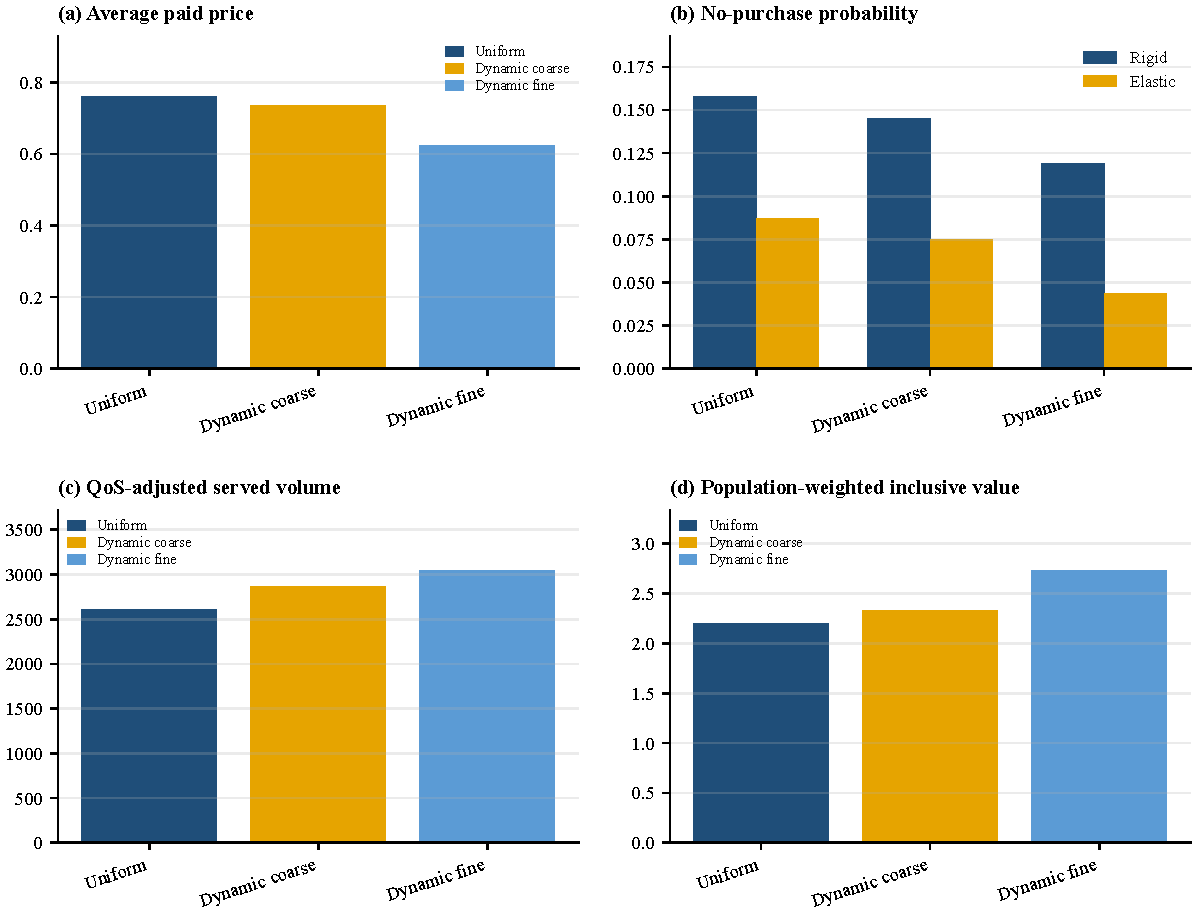
\includegraphics[width=0.9\textwidth]{mechanism_diagnostics.pdf}
\caption{机制诊断。动态快照提高QoS调整后的服务量并降低退出概率，但平均成交价格同步下降，说明QoS改善更接近覆盖率和体验改善，而不是稳定的利润增益。}
\label{fig:mechanism}
\end{figure}

\subsection{剩余重排而非新增供给}

固定算力是本文最重要的约束。动态定价不能增加物理GPU供给，只能改变需求在时间和通道上的分布。图~\ref{fig:mechanism} 给出的诊断和这个判断一致：统一拥塞基准下，QoS调整后的服务量为$2610$；动态粗、细快照分别为$2865$和$3043$。同时，刚性用户退出概率从$0.158$降到$0.145/0.119$，弹性用户退出概率从$0.087$降到$0.075/0.044$。这些数字说明动态策略确实恢复了一部分拥塞损失；混合策略诊断进一步说明，这一QoS方向并不只依赖某个高regret细网格单点。

但这部分改善没有稳定转化为利润。主要原因是价格和数量沿相反方向变化：平均成交价格从$0.761$降至$0.735/0.625$。对厂家利润而言，正向因素包括高峰提价提高单位毛利、低谷降价利用闲置算力，以及削峰后QoS回升带来的有效结算量恢复。反向因素也同时存在：高峰提价会驱动价格敏感需求转向对手、直连或退出；低谷降价会摊薄单位毛利；被挤出高峰的弹性用户也可能转化为净流失。高峰价格收益可能被需求流失抵消，低谷增量服务量也可能被低价薄利抵消。

这不是一个严格的固定总需求定理。本文模型里有退出选项，也有低价时的市场规模扩张项，所以总内部需求会随价格和QoS变化。更准确地说，当前数值结果与一个剩余重排机制相一致：分时定价主要改变需求发生的时段和通道，而没有稳定地产生可由厂家独占的新剩余。

\subsection{QoS损失恢复为何未稳定转化为利润}

QoS从$0.756$回到$0.97$以上，意味着因拥塞导致的无效服务量减少。直观上，这似乎应当增加利润。但有两个因素会削弱这种转化。第一，削峰本身需要转移或压低部分高峰需求：要把利用率从$0.78$压到$0.66$--$0.71$，就必须让一部分高峰用户换时段、换通道或退出。QoS回升带来的有效结算量，可能被价格下降和需求重排抵消。第二，竞争和退出选项限制了涨价空间。两家异质厂家相互竞争，用户又可以直连或退出，任何一家都难以将QoS改善的收益完全转化为自身利润。这部分剩余更可能表现为用户体验改善、完成率改善或价格被竞争压制，而不是厂家利润的稳定上升。

\subsection{运营与监管含义}

动态定价和surge pricing通常被理解为拥塞时期的收入工具。本文的结果更谨慎：在存在竞争、算力固定且用户可以退出的推理服务市场中，分时定价更接近QoS保护工具；至少在当前模型和求解预算下，它没有显示出稳健的正利润增益。对监管者而言，评价分时定价不应只关注其是否提高价格，还应关注其是否减少拥塞和失败请求。对运营者而言，采用分时定价的主要理由应是维护SLA和服务质量，而不是将其视为可靠的收入增长手段。

% ============================================================
\section{局限性}
\label{sec:limitations}

本文有几项局限需要明确说明。所有经济参数（价格敏感度、迁移成本、容量成本、弹性人口占比、退出效用）均为合成标定，尚未使用真实请求轨迹校准。因此，具体百分比只用于说明机制方向，不能作为生产预测。公开API价格只提供价格数量级参照；受控vLLM单卡测量只提供QoS退化形态参照。二者都不能替代真实到达过程、长上下文/多模型/多GPU测量、生产完成率曲线和用户价格弹性估计。

求解层面也存在边界。厂家策略被限制在低维形状族内，本文不声称连续空间的全局最优；细网格单快照的regret仍高，不能作为纯策略均衡结论。双重oracle把有限225点细网格上的混合剖面regret降至$0.203$，但它仍然只是有限候选集上的混合/平均策略诊断，不等于连续策略空间的全局均衡。参数压力测试也有同样边界：它评估已报告策略快照在扰动参数下的表现，而不是在每个参数点重新求解均衡。因此，本文可以更有把握地保留QoS改善方向，但仍不将利润、厂家动态强度或连续空间均衡性质写成定理。

范围限制还包括市场结构和后端测量。本文只研究两厂家、单中间商；更多厂家、多中间商、长期容量合约和模型路由之间的复杂互动尚未纳入。QoS退化使用合成的sigmoid曲线，真实后端的完成率和延迟曲线仍需要用受控测量或生产轨迹重新标定。最后，利润不呈现稳健正增益这一发现依赖当前的固定算力、竞争结构和需求设定；如果需求总量本身对价格更敏感，或者算力短期内可调，结论可能不同。

% ============================================================
\section{结论}
\label{sec:conclusion}

本文研究固定算力约束下，分时动态定价能否改善推理服务的服务质量。为此，本文构建了一个包含竞争异质双厂家、可路由中间商、两类用户和退出选项的市场模型，并用低维形状参数化与虚拟博弈求解厂家Nash竞争。虚拟博弈缓解了朴素最优响应在拥塞区间的极限环振荡，使求解过程具有可复现性。

经过粗、细两套网格、细网格混合策略诊断和局部参数压力测试，本文得到一个有边界但更具证据支撑的结论：拥塞时分时动态定价显示出削峰和QoS改善方向，将最低QoS从$0.756$提高到$0.97$左右或以上；双重oracle在完整225点细网格上将混合剖面的最大regret降至$0.203$，参数扰动下QoS增益也保持为正。利润结果则不稳健，符号随求解对象和网格变化而变化。因此，本文不主张分时动态定价能够稳定提高利润。本文用剩余重排解释这一现象：在固定算力、竞争和退出选项约束下，价格变化带来的收益容易被需求外流、低价薄利和剩余转移抵消。对运营和监管而言，分时定价更适合作为服务质量管理工具，而不是收入增长工具。后续工作需要引入真实轨迹校准，在连续策略空间或更大候选集上验证低exploitability，并扩展到更多厂家和中间商。

\section*{代码与工件可用性}
削峰填谷仿真模块为\path{pricing_sim/peak_shaving_config.py}、
\path{pricing_sim/peak_shaving_market.py}和
\path{pricing_sim/peak_shaving_equilibrium.py}。主要实验入口包括：
\begin{itemize}[leftmargin=2em]
  \item \path{experiments/run_peak_shaving_experiments.py}：非拥塞主实验；
  \item \path{experiments/run_peak_shaving_congested_fp.py}：拥塞虚拟博弈；
  \item \path{experiments/run_fp_dynamic_converge.py}：regret收敛与断点续跑；
  \item \path{experiments/run_peak_shaving_robustness.py}：QoS形态、退出效用、跨种子；
  \item \path{experiments/run_peak_shaving_mixed_oracle.py}：细网格混合策略诊断；
  \item \path{experiments/run_peak_shaving_parameter_sweep.py}：参数压力测试；
  \item \path{experiments/build_peak_shaving_measurement_anchor.py}：受控vLLM QoS测量锚点。
\end{itemize}
机制诊断和图表由\path{experiments/build_peak_shaving_diagnostics.py}从既有策略工件重建。
机器可读工件均在\path{artifacts/peak_shaving/}下，子目录分别为
\path{20260618/}、\path{20260619/}和\path{20260619_submission/}。图表均在
\path{figures/}下，子目录为\path{peak_shaving_diagnostics/}和
\path{peak_shaving_submission/}。参数、网格设置、工件映射和复现命令见补充材料
\path{peak_shaving_dynamic_pricing_supplement_2026-06-19.tex}。

\small
\bibliographystyle{unsrtnat}
\bibliography{verified_refs}

\end{document}
